\documentclass[11pt,a4paper]{article}
\usepackage[T1]{fontenc}
\usepackage[utf8]{inputenc}
\usepackage{lmodern}
\usepackage[margin=1in]{geometry}
\usepackage{graphicx}
\graphicspath{{figures/}{../docs/}}
\usepackage{booktabs}
\usepackage{amsmath}
\usepackage{xcolor}
\usepackage{caption}
\captionsetup{font=small,labelfont=bf}
\usepackage{enumitem}
\usepackage[hidelinks]{hyperref}
\usepackage{cleveref}
\usepackage{parskip}
\usepackage{longtable}
\usepackage{tikz}
\usetikzlibrary{arrows.meta,positioning,fit,backgrounds}
\setlength{\emergencystretch}{1.5em}
\definecolor{flblue}{HTML}{4F81BD}
\definecolor{agred}{HTML}{C0504D}

\title{\textbf{fedOPD: Cross-Silo Federated Forecasting and Agentic\\ Capacity Planning for NHS Referral-to-Treatment Demand}\\[0.4em]
\large System Report --- Architecture, Method, and First Working Prototype}
\author{Nilesh Sarkar \\ \small fedOPD project}
\date{16 July 2026}

\begin{document}
\maketitle

\begin{abstract}
This report documents \emph{fedOPD}, a working prototype that forecasts NHS outpatient
Referral-to-Treatment (RTT) demand under privacy constraints and turns those forecasts into
capacity and allocation decisions. The system is built as \textbf{two coupled planes} over the NHS
provider hierarchy: a \emph{federated-learning plane} in which each NHS trust trains a shared
per-department demand forecaster without its raw data ever leaving the site, and an \emph{agentic
plane} that consumes the forecasts together with the live waiting-list state and recommends where
capacity should be added. Everything reported here is reproducible and traceable: each figure and
number derives from a committed artefact and a logged, gated build step. The forecasting plane trains
across \textbf{117 NHS-trust clients} and \textbf{17 clinical departments} ($1{,}544$ monthly series,
$108{,}065$ training windows) and is measured on a fixed 12-month back-test of $18{,}191$
(series, month) points against a strong persistence baseline. The headline result is honest rather
than inflated: federated learning with per-client personalisation reaches a macro-mean sMAPE of
$16.24\pm0.07$, \textbf{beating isolated per-trust training by $0.66$ points} (far outside seed noise)
and matching the naive-$t{-}1$ bar ($16.34$), while the privacy-ignoring centralised upper bound
($15.81$) confirms there is learnable shared structure beyond persistence. A hand-written federated
loop and a Flower implementation agree to within $0.004$ sMAPE. The agentic prototype builds a
validated demand$\rightarrow$backlog$\rightarrow$capacity flow model from the same files, and for
2026-03 flags \textbf{969 of $1{,}509$} panel services as breaching the 18-week standard and computes
the additional monthly throughput each Integrated Care Board would need to recover.
\end{abstract}

\tableofcontents
\clearpage

\section{The operational problem and why this design}\label{sec:intro}
NHS England publishes, every month, how many patients are waiting for consultant-led treatment, by
provider and by treatment function. Three flows govern each service: \emph{demand} (new referral
clocks started), \emph{throughput} (clocks stopped by treatment), and the \emph{backlog} (patients
still waiting). Planning capacity against demand --- clinics, workforce, and where to direct
investment --- is an operations-research problem, not a clinical one. The object we learn is a
per-department \emph{demand forecaster}; we never touch patient records.

Two facts shape the architecture. First, every trust reports the same signal in the same schema, so
the many providers are natural collaborators on one forecasting task --- but their operational data
is governed locally and cannot simply be pooled. \textbf{Federated learning} resolves this: each
trust is a cross-silo client that trains a shared model on its own data and exchanges only model
updates. Second, a forecast is not a decision. A demand number becomes useful only when combined with
the current waiting list and turned into a staffing or allocation recommendation --- the
\textbf{agentic plane}. The two planes branch on provider type in exactly one place: capacity is
\emph{allocated} to NHS trusts (which are directable), whereas independent providers can only be
\emph{commissioned}. This prototype scopes both planes to NHS trusts.

\section{System architecture}\label{sec:arch}
\Cref{fig:arch} shows the two planes over one hierarchy (NHS England $\rightarrow$ region
$\rightarrow$ Integrated Care Board (ICB) $\rightarrow$ trust $\rightarrow$ department). In the
learning plane the global model flows down and model updates flow up, aggregated by a coordinator. In
the agentic plane, forecasts feed a decision engine whose allocations flow down and whose resource
requests flow up. The region tier is not present in the RTT files and is left as an external
attribution step; all results here use the trust and ICB tiers, which are in the data.

\begin{figure}[htbp]
\centering
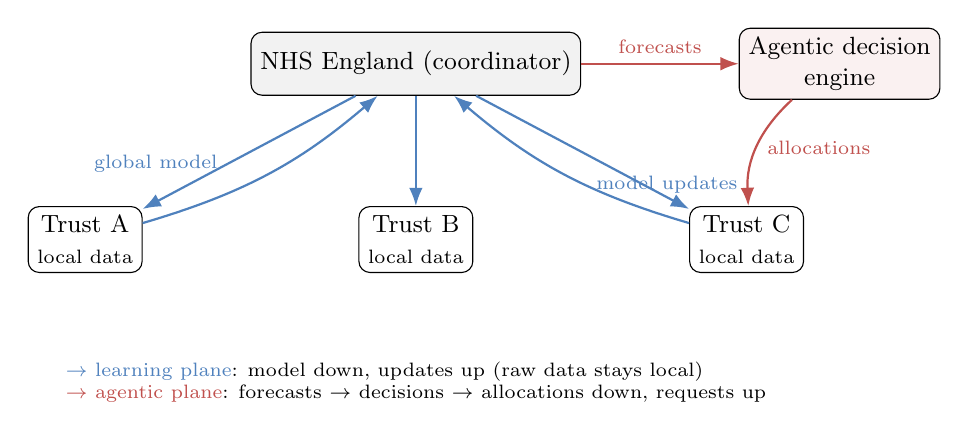
\begin{tikzpicture}[font=\small,>=Latex,node distance=6mm,
  box/.style={draw,rounded corners,minimum height=8mm,align=center,fill=white},
  hq/.style={box,fill=black!5}]
\node[hq] (hq) {NHS England (coordinator)};
\node[box,below=14mm of hq,xshift=-42mm] (t1) {Trust A\\\scriptsize local data};
\node[box,below=14mm of hq] (t2) {Trust B\\\scriptsize local data};
\node[box,below=14mm of hq,xshift=42mm] (t3) {Trust C\\\scriptsize local data};
% FL plane arrows
\draw[->,flblue,thick] (hq) -- node[left,pos=.6,font=\scriptsize]{global model} (t1);
\draw[->,flblue,thick] (t3) to[bend left=12] node[right,pos=.4,font=\scriptsize]{model updates} (hq);
\draw[->,flblue,thick] (hq) -- (t2);
\draw[->,flblue,thick] (hq) -- (t3);
\draw[->,flblue,thick] (t1) to[bend right=12] (hq);
% agentic plane
\node[box,fill=agred!8,right=20mm of hq] (ag) {Agentic decision\\engine};
\draw[->,agred,thick] (hq) -- node[above,font=\scriptsize]{forecasts} (ag);
\draw[->,agred,thick] (ag) to[bend right=25] node[right,font=\scriptsize]{allocations}(t3);
\node[align=left,below=10mm of t2,font=\scriptsize] (leg)
  {\textcolor{flblue}{$\rightarrow$ learning plane}: model down, updates up (raw data stays local)\\
   \textcolor{agred}{$\rightarrow$ agentic plane}: forecasts $\rightarrow$ decisions $\rightarrow$ allocations down, requests up};
\end{tikzpicture}
\caption{The two coupled planes over the provider hierarchy. Raw referral data never leaves a trust;
only model parameters (up) and the global model / allocations (down) move.}
\label{fig:arch}
\end{figure}

\section{Data, variables, and assumptions}\label{sec:data}
\subsection{Sources and the two derived tables}
One public source is used: NHS England Consultant-led RTT waiting-time ``Full CSV'' extracts, 96
consecutive monthly files spanning \textbf{2018-04 to 2026-03} (eight financial years, bracketing the
COVID collapse and recovery). Two tables are derived from it with identical provider filters (keep NHS
trusts \texttt{R\#\#}; drop the aggregate specialty \texttt{C\_999}; sum over commissioner):
\begin{itemize}[nosep]
  \item \textbf{Canonical demand} \texttt{[date, branch, dept, demand]} --- $227{,}344$ rows; the
        learning target, from \texttt{Part\_3} (new RTT clocks), verified against published national
        totals in four sentinel months (4/4).
  \item \textbf{Operational flow} \texttt{[date, branch, dept, demand, completed, backlog, breach18]}
        --- $231{,}508$ rows; the agentic state, adding throughput (\texttt{Part\_1A+1B}), the
        incomplete-pathway stock (\texttt{Part\_2}), and the count of waiters over 18 weeks
        (\texttt{Part\_2} wait bands $\geq 18$).
\end{itemize}

\subsection{Every assumption in one place}
\Cref{tab:assump} lists every modelling assumption and fixed variable, so nothing is implicit.

\begin{longtable}{@{}p{0.30\linewidth} p{0.30\linewidth} p{0.34\linewidth}@{}}
\caption{Assumptions and fixed variables.}\label{tab:assump}\\
\toprule
Variable / assumption & Value & Rationale \\ \midrule \endfirsthead
\toprule Variable / assumption & Value & Rationale \\ \midrule \endhead \bottomrule \endfoot
Window (input lags) & 12 months & lag-1 autocorrelation $0.80$ dominates; one full year \\
Forecast horizon & 1 month ahead & operational planning cadence \\
Demand signal & \texttt{Part\_3 Total All} & new RTT clocks = incoming demand \\
Client (silo) & one NHS trust & data governed at trust level \\
Balanced panel & 125 trusts (all 96 months) & clean time split, no imputation \\
Department roster & 17 (span all 96 months, $\geq 50\%$ panel coverage) & stable clinical specialties \\
Federated clients & \textbf{117} (of 125) & 8 trusts offer only off-roster services \\
Train / test split & 2018-04..2025-03 / 2025-04..2026-03 & last 12 months held out (a full seasonal cycle) \\
Scaling & per-series $z$-score, train-only & heavy skew; fitted excluding flagged months \\
Regime features & COVID 2020-03..2021-03; strike 2022-12..2023-12 & shared shocks, kept not deleted \\
Target formulation & \emph{delta} (predict $y_t - y_{t-1}$) & naive-anchored; beats \emph{level} \\
Model & MLP $33\!\to\!64\!\to\!32\!\to\!1$ ($4{,}289$ params) & small; monthly data is short \\
FL rounds / local epochs & 40 / 1 & convergence (loss still descending) \\
Metric & sMAPE on raw counts, per series then macro-mean & scale-free; small-series honest \\
18-week standard & $4.14$ months (Little's law) & RTT constitutional standard \\
Backlog recovery horizon & 12 months & agentic burn-down target \\
\bottomrule
\end{longtable}

\subsection{Who the clients are}
The federated panel is \textbf{117 NHS trusts $\times$ 17 clinical departments}. Of the 125
balanced-panel trusts, eight contribute no eligible series (they run only off-roster services, e.g.
cancer-specialist Clatterbridge, paediatric Great Ormond Street, and six mental-health/community
trusts). This yields $1{,}528$ evaluable series plus $16$ ``train-only'' series (active but with an
interior gap in the test year: they contribute gradient signal but are not scored), giving
$1{,}544$ training series, $108{,}065$ training windows and $18{,}191$ test points. Each series carries
$33$ features: 12 scaled demand lags, month sine/cosine, a COVID flag, a 2023-strike flag, and a
17-way department one-hot.

\section{Method: the forecasting plane}\label{sec:method}
\subsection{Forecaster and interface}
The model sits behind a four-call interface --- \texttt{get\_params}, \texttt{set\_params},
\texttt{train\_epochs}, \texttt{predict} --- so the federated loop never touches its internals and the
network could be swapped without changing the aggregation. We use the \emph{delta} formulation:
the model predicts the month-on-month change and reconstructs the level as
$y_{t-1} + \widehat{\Delta}$. This is \emph{naive-anchored}: a model predicting zero change reproduces
the persistence baseline exactly, so it starts at the bar and can only add skill. Every result passed
gates for parameter round-trip, single-series overfitting, determinism, and exact naive anchoring.

\subsection{Federated methods}
\begin{itemize}[nosep]
  \item \textbf{Local-only} --- each trust trains alone (compute-matched, and given a fair fight:
        train-tail early stopping, weight decay, small-client batch).
  \item \textbf{Centralised} --- all data pooled; the privacy-ignoring upper bound.
  \item \textbf{FedAvg} --- broadcast global model, each client trains one local epoch, example-count
        weighted aggregation, 40 rounds.
  \item \textbf{FedProx} --- FedAvg plus a proximal term $\tfrac{\mu}{2}\lVert w-w_{\text{global}}\rVert^2$,
        $\mu\in\{0.001,0.01,0.1\}$.
  \item \textbf{Personalisation (+ft)} --- fine-tune the final global model per client with tail-val
        early stopping (a thin-client guard).
  \item \textbf{Selective} --- per client, pick the best of \{naive, local, global+ft\} on a held-out
        validation slice; reported as an honest negative (below).
\end{itemize}

\subsection{The bar}
The persistence baseline naive-$t{-}1$ is scored on \emph{exactly} the same $18{,}191$ points and
aggregation as every model. On the panel it is $16.34$ macro-mean (median $12.92$, volume-weighted
$12.35$). We verified the metric by reproducing the earlier EDA baseline on its original scope
($12.6/15.7$, within tolerance) before trusting any model number.

\section{Results: forecasting}\label{sec:results}
\Cref{tab:methods} and \Cref{fig:methods} give the headline. The verdict is stated against seed noise.

\begin{table}[htbp]\centering
\caption{Forecast accuracy (delta target), macro-mean sMAPE over 5 seeds. Lower is better; the bar is
naive-$t{-}1$ at $16.34$.}\label{tab:methods}
\begin{tabular}{lrrl}
\toprule
Method & macro-mean $\pm$ std & median & vs bar \\ \midrule
seasonal-naive $t{-}12$      & $23.26$          & $16.39$ & $+6.92$ \\
local-only (fair fight)      & $16.90\pm0.05$   & $12.11$ & $+0.56$ (loses) \\
selective per-client         & $16.83$          & $12.04$ & $+0.49$ (loses) \\
FedAvg                       & $16.35\pm0.06$   & $11.20$ & ties \\
FedProx ($\mu{=}.001$)       & $16.31\pm0.07$   & $11.21$ & ties \\
\textbf{FedAvg + personalise}& $\mathbf{16.24\pm0.07}$ & $11.39$ & $-0.10$ (ties) \\
FedProx + personalise        & $16.22\pm0.09$   & $11.41$ & $-0.12$ (ties) \\
centralised (upper bound)    & $15.81\pm0.39$   & $11.06$ & $-0.53$ (beats) \\
\bottomrule
\end{tabular}
\end{table}

\begin{figure}[htbp]\centering
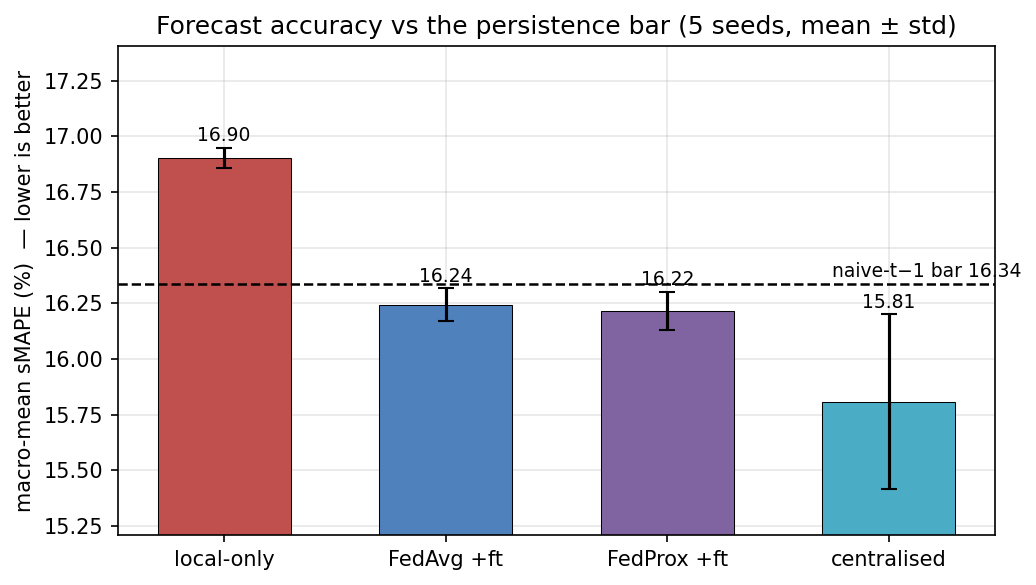
\includegraphics[width=0.72\linewidth]{fc_methods.png}
\caption{Forecast accuracy against the persistence bar (5 seeds, mean $\pm$ std).}\label{fig:methods}
\end{figure}

Four things are true at once, and we report all four:
\begin{enumerate}[nosep]
  \item \textbf{Federation decisively beats isolation.} FedAvg+personalise minus local-only is
        $-0.66$ points, far outside the $\pm0.07$ seed noise. The privacy-preserving setup recovers
        most of the local$\rightarrow$centralised gap \emph{without any raw data leaving a site}.
  \item \textbf{Against plain persistence the verdict is honest.} On macro-mean the federated model
        ties the naive bar; monthly series with 84 training points are exactly where neural
        forecasters struggle to beat persistence. On the \emph{median} series every neural method
        wins clearly ($11.2$--$11.4$ vs $12.92$): the macro-mean is dominated by a volatile
        small-series tail where naive is near-optimal.
  \item \textbf{There is learnable shared signal.} The centralised upper bound beats the bar
        ($15.81$), so co-movement across trusts is real structure; the remaining fed$\leftrightarrow$
        central gap ($\sim0.4$) is the measurable price of not pooling.
  \item \textbf{Personalisation and prox help modestly}; strong prox hurts (expected under full
        cross-silo participation); per-client \emph{selection} does not help (\Cref{fig:methods}
        omits it as a line; the validation-window signal does not transfer to the test year).
\end{enumerate}

\begin{figure}[htbp]\centering
\begin{minipage}{0.49\linewidth}\centering
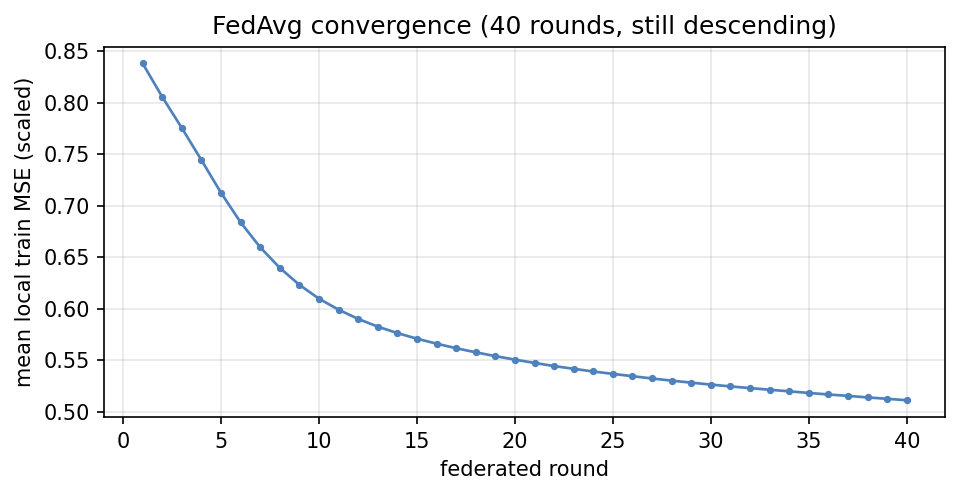
\includegraphics[width=\linewidth]{fc_loss.png}\end{minipage}\hfill
\begin{minipage}{0.49\linewidth}\centering
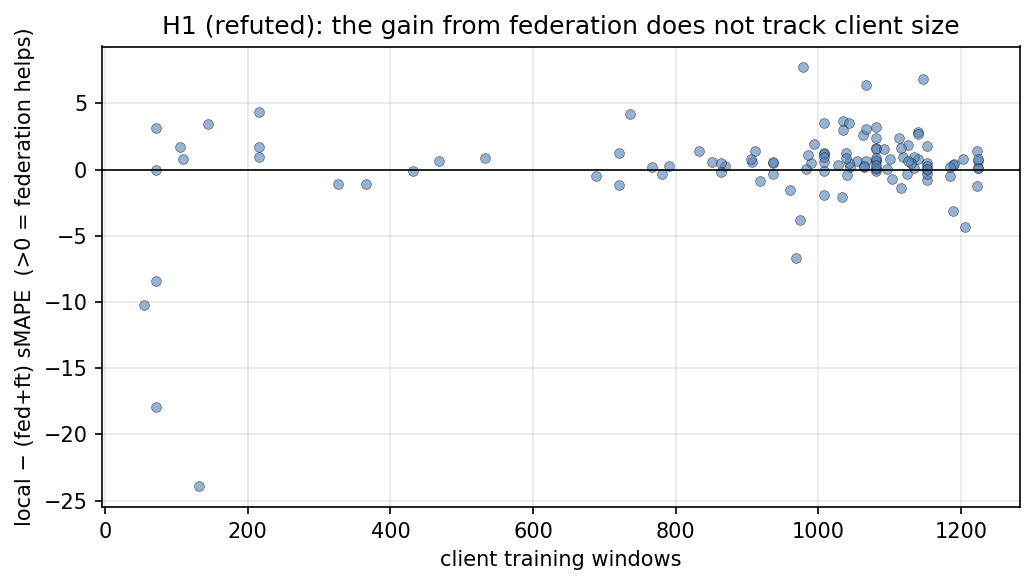
\includegraphics[width=\linewidth]{fc_h1.png}\end{minipage}
\caption{Left: FedAvg convergence over 40 rounds (still descending). Right: the pre-registered
hypothesis H1 --- that the gain from federation grows for smaller clients --- is \textbf{refuted}
(Spearman $\rho=0.038$, $p=0.68$); gains concentrate in mid-size clients, and the thinnest are better
off local (early stopping collapses them onto the near-optimal naive anchor).}
\label{fig:diag}
\end{figure}

\subsection{Robustness}
\Cref{fig:sens} runs the open supervisor choices as a sensitivity table, each variant scored against
its \emph{own} recomputed bar. Including Neurosurgery (roster 18) costs nothing; including the
``Other'' X-codes (all 24) breaks nothing; results are robust across panel strictness (125/139/146
trusts). So the roster/threshold decisions are not accuracy-driven --- they rest on taxonomy stability
and on whether a service is one the agentic layer could allocate to. A hand-written and a Flower
FedAvg agree to \textbf{$0.004$} sMAPE, confirming the design runs on a standard FL framework.

\begin{figure}[htbp]\centering
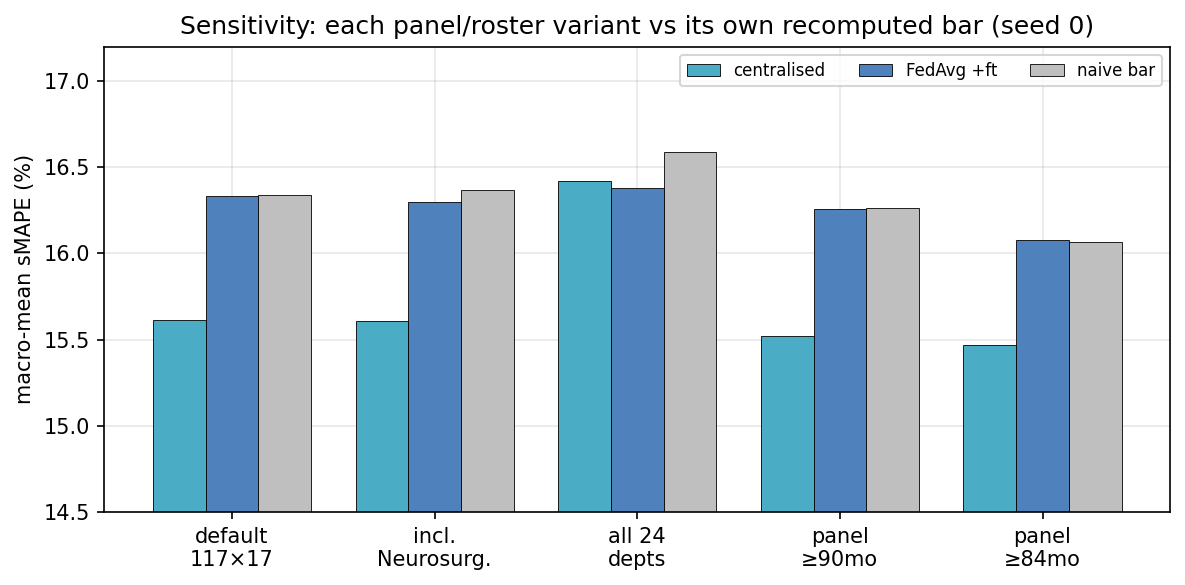
\includegraphics[width=0.8\linewidth]{fc_sensitivity.png}
\caption{Sensitivity of centralised and FedAvg+ft to the panel and roster choices (seed 0), each vs
its own recomputed naive bar.}\label{fig:sens}
\end{figure}

\section{Method and results: the agentic plane}\label{sec:agentic}
\subsection{From a forecast to a decision}
The decision engine is transparent operations research --- the policy an LLM agent would execute. For
each trust$\times$department$\times$month it holds four state variables: the federated demand forecast
$\widehat{D}$, the observed backlog $B$, a trailing-12-month throughput baseline $C_{\text{base}}$, and
the count of $>18$-week waiters. By Little's law the mean wait in months is
$\approx B / C$, so the 18-week standard ($4.14$ months) implies a sustainable backlog
$B^\star = 4.14\,\widehat{D}$. The throughput required to absorb demand \emph{and} burn the excess
backlog over a 12-month horizon is
\[
C_{\text{req}} \;=\; \widehat{D} \;+\; \frac{\max(0,\; B - B^\star)}{12},
\qquad
\text{capacity gap} \;=\; C_{\text{req}} - C_{\text{base}} .
\]
A positive gap is a staffing signal (allocate more capacity); a RED/AMBER/GREEN status follows from
the current implied wait ($\geq18$, $12$--$18$, $<12$ weeks). Gaps sum up the hierarchy
(trust $\rightarrow$ ICB $\rightarrow$ national) to say \emph{where} capacity should be directed.

\subsection{The flow model is validated}
The engine rests on the identity $B_t \approx B_{t-1} + D_t - C_t$. Nationally it holds to a
\textbf{3.8\%} median error; per client$\times$month it is noisier but clearly signed
(\Cref{fig:flowval}). \Cref{fig:flow} shows the operational context the forecasts feed into: demand
collapsed in 2020 and recovered, but throughput never caught up, so the backlog climbed to
$\sim$$6.6$M pathways, of which \Cref{fig:breach} shows $\sim$$2.3$M are now waiting over 18 weeks ---
the target the agentic layer exists to reduce.

\begin{figure}[htbp]\centering
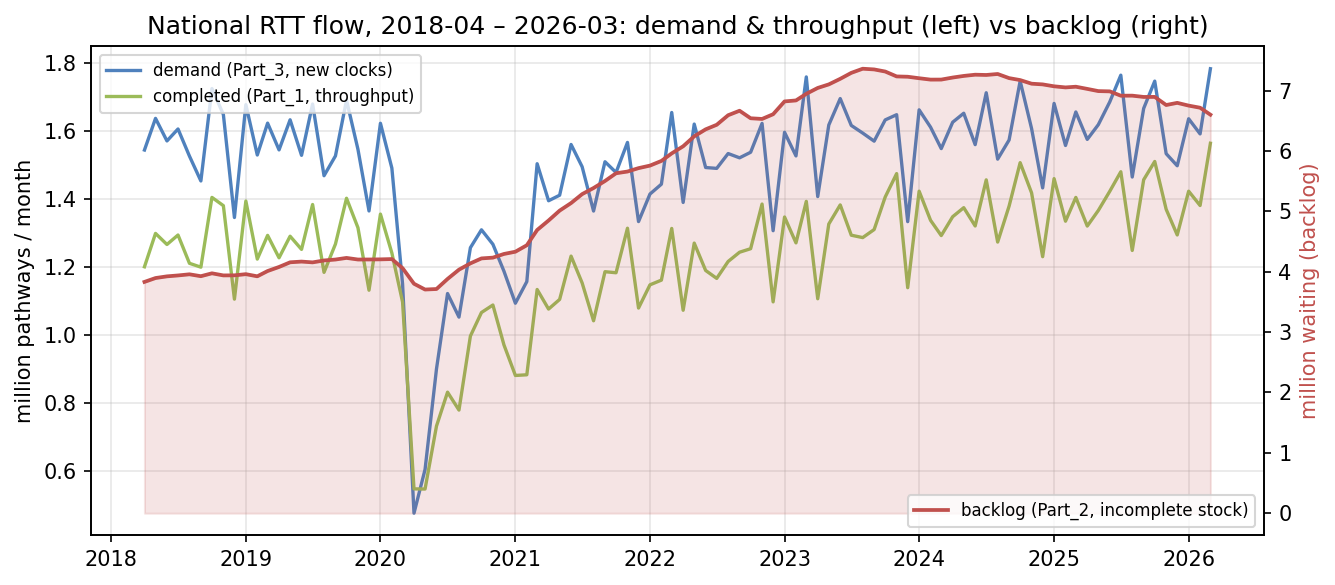
\includegraphics[width=0.92\linewidth]{ag_flow_national.png}
\caption{National RTT flow: demand and throughput (left axis) against the incomplete-pathway backlog
(right axis). Throughput never overtakes demand post-recovery, so the backlog grows.}\label{fig:flow}
\end{figure}

\begin{figure}[htbp]\centering
\begin{minipage}{0.60\linewidth}\centering
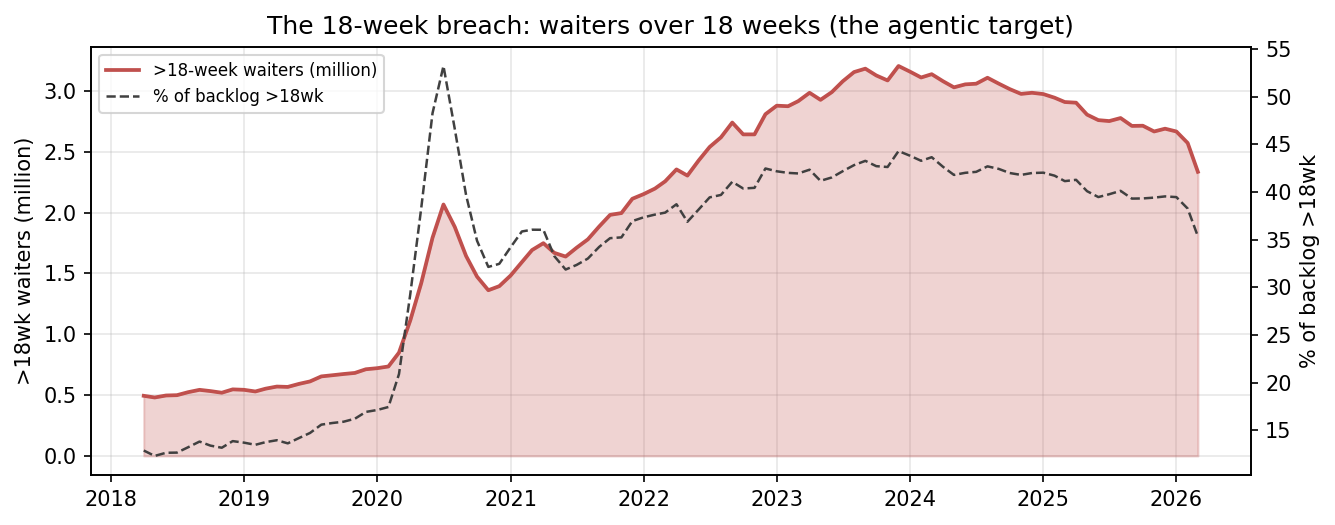
\includegraphics[width=\linewidth]{ag_breach.png}\end{minipage}\hfill
\begin{minipage}{0.38\linewidth}\centering
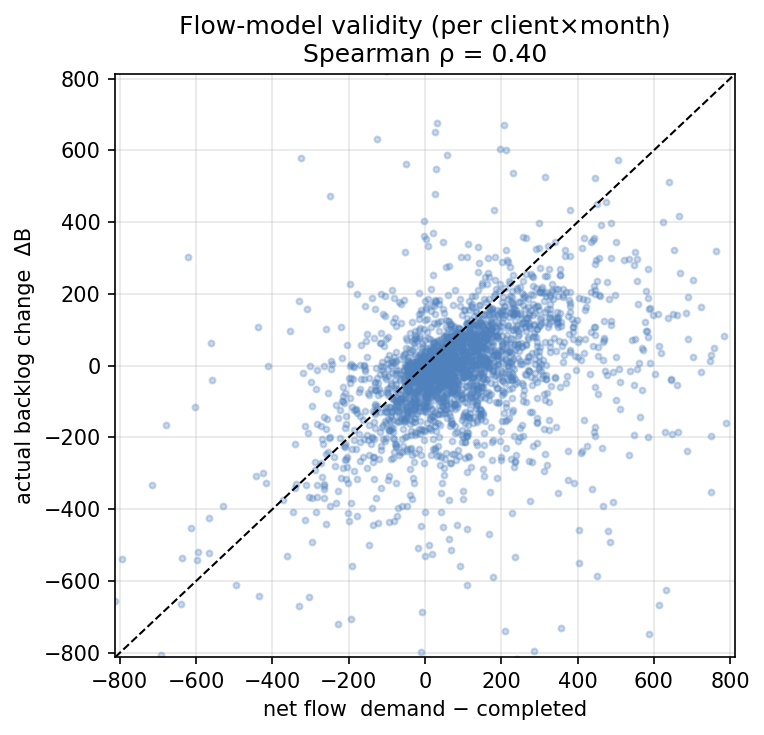
\includegraphics[width=\linewidth]{ag_flow_validity.png}\end{minipage}
\caption{Left: the $>18$-week breach --- the quantity the decision engine targets. Right: the flow
model's validity per client$\times$month (net flow vs actual backlog change).}\label{fig:breach}
\label{fig:flowval}
\end{figure}

\subsection{The decision snapshot (2026-03)}
Applied to the federated panel ($1{,}509$ services with a full flow history), the engine flags
\textbf{969 RED, 322 AMBER, 218 GREEN}. RED services --- those the Little's-law proxy implies are waiting $>18$ weeks --- carry the highest
\emph{actual} $>18$-week share of their backlog, measured independently from the \texttt{Part\_2} wait
bands (\Cref{fig:rag}, right); the proxy therefore agrees with the ground-truth waiting-time data. Summed to ICB level, the engine ranks
where additional monthly throughput is most needed (\Cref{fig:alloc}); nationally the panel needs on
the order of \textbf{$216$k additional pathways per month} to move onto a recovery trajectory.
\Cref{fig:client} traces one service end to end: the federated forecast, the observed backlog, and the
resulting monthly capacity gap the agent would act on.

\begin{figure}[htbp]\centering
\begin{minipage}{0.54\linewidth}\centering
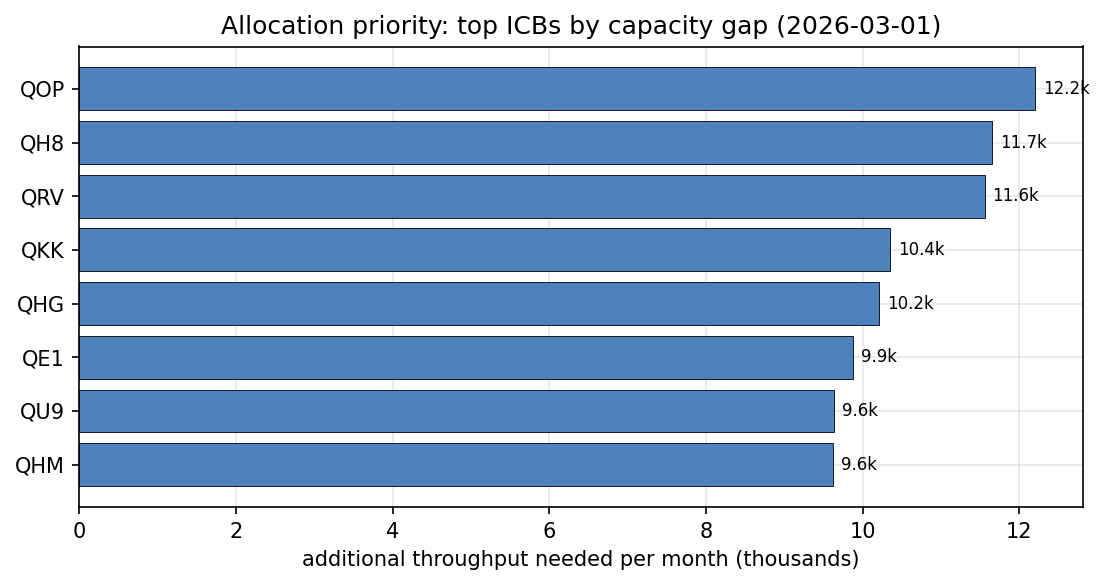
\includegraphics[width=\linewidth]{ag_icb_alloc.png}\end{minipage}\hfill
\begin{minipage}{0.44\linewidth}\centering
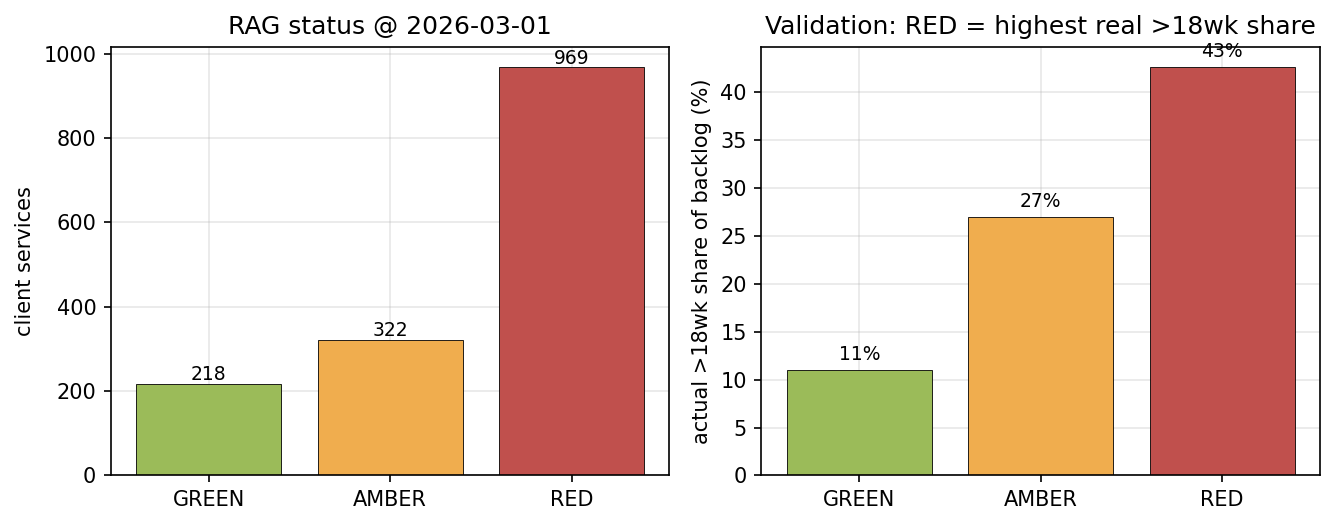
\includegraphics[width=\linewidth]{ag_rag.png}\end{minipage}
\caption{Left: allocation priority --- ICBs ranked by the additional monthly throughput their
services need (2026-03). Right: RAG status distribution, and the validation that RED services carry
the highest \emph{actual} $>18$-week backlog share, measured independently from the wait bands.}\label{fig:alloc}\label{fig:rag}
\end{figure}

\begin{figure}[htbp]\centering
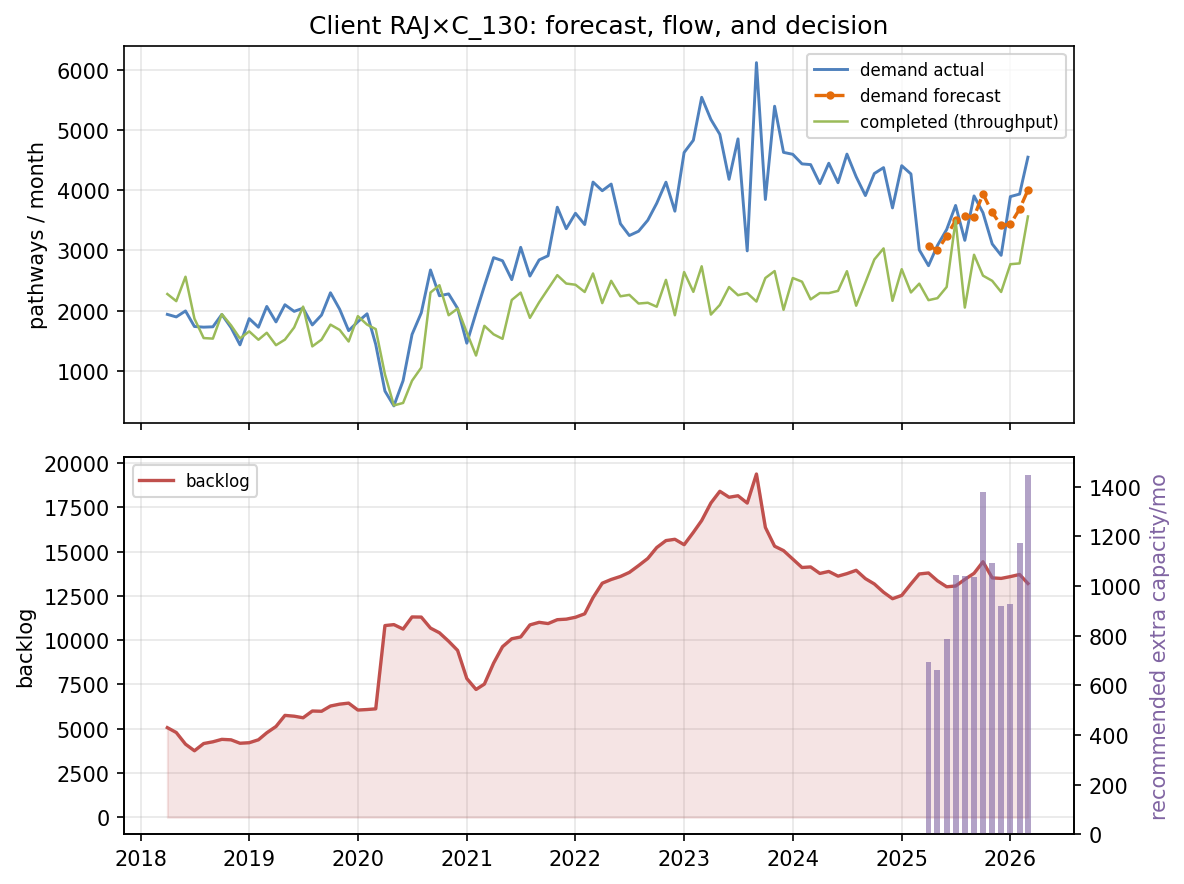
\includegraphics[width=0.85\linewidth]{ag_client_decision.png}
\caption{One client service end to end: demand forecast vs actual and throughput (top); backlog and
the recommended monthly capacity gap the agent acts on (bottom).}\label{fig:client}
\end{figure}

\section{Discussion: what is and is not defensible}\label{sec:disc}
The claims we stand behind are narrow and evidenced. \emph{Federation beats isolated training} by a
margin far outside seed noise, with no raw data leaving any site --- the core privacy-vs-utility
result. \emph{There is shared structure to learn}, shown by the centralised model beating persistence
and by strong cross-trust co-movement. \emph{On this operational metric, the federated model matches a
strong persistence baseline} rather than crushing it --- which is the honest outcome for short monthly
series and is stated plainly, with the median-series win and the centralised headroom both reported.
The agentic layer is a \emph{transparent, validated decision policy}, not a black box: every step is a
named quantity a planner can audit.

\textbf{Limitations, stated openly.} (i) The macro-mean is dominated by a small-series tail where
naive is near-optimal; the win lives in the median and in the centralised bound. (ii) Per-client model
selection did not transfer across the year and is reported as a negative. (iii) The per-service flow
identity is noisy (clock pauses, removals, revisions); the agentic engine is therefore most reliable
at ICB and national aggregation, where noise averages out. (iv) The region tier is not in the data.
(v) Forecasts are one month ahead; multi-month planning needs recursive or direct multi-horizon
forecasting. None of these is hidden in the numbers.

\section{Reproducibility and roadmap}\label{sec:repro}
Every number traces to a committed artefact: the frozen panel and dataset (\texttt{results/*.json}),
one JSON per model run (config, seed, git SHA, duration), the flow table, and the agentic decision
parquet. The build ran in ten gated steps (each logged in \texttt{docs/BUILD\_LOG.md}); the whole
programme is CPU-minutes and reproduces with \texttt{bash scripts/run\_grid.sh}, then
\texttt{python -m src.fedopd.agentic} and \texttt{-m src.fedopd.make\_figures}. The EDA foundation is
tagged \texttt{eda-v2}; the forecasting build \texttt{build-v1}.

\textbf{Next steps, in priority order:} (1) per-client model \emph{selection on a rolling window} to
convert the median-series win into a macro-mean win; (2) multi-horizon forecasting to drive
multi-month capacity plans; (3) the region attribution lookup to complete the hierarchy; (4) an
LLM-orchestrated agent wrapping the (already validated) decision policy, with the trust-vs-independent
allocate/commission branch; (5) a legibility ``scenario panel'' (a few regions $\times$ hospitals
$\times$ departments) so the decisions are inspectable without reading a $117\times17$ grid.

\end{document}
